\chapter{Task Description}

\section{Task Description and Overview}

%Sushi mente hun ikke forsto hensikt med kap 2. Skal vi skrive om ingressen her? Syntes selv den egentlig er grei nok
The first step in our development process was to get a brief overview of
our complete system. To do this, we have followed a conventional style
of designing UML use cases together with a textual description. From
reading this chapter, the reader should be able to understand how our
end product works. Also, reading this chapter will be important to
understand the other chapters in this report. The assumptions and
constraints that affected our process are also discussed in section
X.X. 

\subsection{Assignment}
According to our customers, ``IDI
Open'''s previous solution was
cumbersome to use. Our assignment was to create a replacement system
that would be easier to administer.
This included replacing both front and back-end systems. In replacing
the old solution, we did not need to implement features that were not
available from the old system. 

The features of the old solution, in a nutshell, are given below. A more
detailed overview will be given in section X.X.
\begin{itemize}
\item Website to inform about the contest to the public
\item Team-registration and scoring
\item Ability for users to upload code, that would be compiled and
executed by the server
\end{itemize}

We were given access to the code for the old solution. The customers
felt that this code was cluttered, but we could re-use components
wherever we wanted. However, it was important that we did this in an
uncluttered way, such that other developers could easily understand the
new solution.

\subsection{Branding our Product}

Since we were delivering an end product to a real customer, we wanted to
present ourselves as a real company. We chose the name
``GentleCoding'' as our
representative name. This was used to name our repositories, email
lists and other medium communicated with external parties.

The term ``Gentle'' is supposed to
represent our calm approach to problems. It is also similar to ``Gentleman'',
which reminds of quality and good conduct. Furthermore, it is easy to interpret
and remember.

Since we were developing a new system, we also wanted to brand our
product. We wanted to keep it logical and simple, so we decided on
``GentleIDI''. Consequently,
GentleIDI will be used to refer to our end product throughout the rest of the report.
\subsection{Assumptions and Constraints}


To define what is satisfactory, we have made some assumptions and
defined some constraints. Table X.X should make it easier to understand
how we have reasoned our system design. 

\begin{table}
\tablehead{}
\begin{supertabular}{|m{2.0879598in}|m{2.0879598in}|m{2.0879598in}|}
\hline
Assumption/Constraint &
Why &
Implication\\\hline
The system will be maintained by people who have experience with
computers &
People that are involved with any programming contest are typically
programmers themselves. &
User design, words and definitions can be made more technical. Error
messages can be explained using computer lingo. \\\hline
The system will be used and maintained for {\textgreater} 5 years &
Customer{}-constraint: they do not want to spend too much time
developing new products, so maintenance is preferred. &
\ The code should be written in a modular, extensible way with clear
documentation.\\\hline
The customers, IDI Open, are students near/at Gl�shaugen &
 &
High availability for customer meetings and reviews.\\\hline
The developers will maintain a 20 hour a week work ethic throughout the
project{}-duration of 20 weeks[TODO: update] &
To finish the product (on{}-time) &
The set of requirements should not require more than 20 hours of work
per week per developer, in order to complete.\\\hline
Our system should be user{}-friendly &
Our solution features a web interface available to everyone. Ideally,
any person should be be comfortable with the user interface. &
\\\hline
Our end product will be open sourced &
To ensure quality, and let other volunteers contribute to the code
repository &
No proprietary third party modules can be used. \ We cannot copyright
our own material. \\\hline
The final solution must run on Linux{}-computer &
This is the choice of OS by NTNU, which is responsible for technical
support and server access &
Linux{}-compliant solution\\\hline
We are allowed to use whatever third party plugin we want, as long as it
is free and has no copyright{}-conflict &
Speed up development &
Speed up development\\\hline
\end{supertabular}
\end{table}

Do note that the implications in table X.X were not necessarily upheld.
Rather, they were used as initial bounds to permit leeway. For example,
imposing that third party plugins will speed up development does not
mean that we would alway prioritize software re-use.

Roles and Their Definitions
Usergr\oups
Within the application-domain of
``gentleidi'' there are different
groups of users. Each group has different levels of access control, and
once a user is made a member of that group, they inherit those rights.
A user may have membership in all groups. A privileged user is someone
who is manually given elevated permissions. Table X.X shows the
different roles and their available actions. Further elaborations on
each group will also be given in later sections, but table X.X should
suffice for an overview.

\begin{table}
\tablehead{}
\begin{supertabular}{|m{1.7025598in}|m{4.39006in}|}
\hline
Role &
Description\\\hline
Admin &
Privileged. An admin can modify all the available settings of the
system\\\hline
Judge &
Privileged. Similar to an admin account, but with a limited set of
actions: answering questions (clarification system), upload tasks to be
solved, solutions to those tasks, upload incorrect answers (e.g.\ answers
that will provide penalty).\\\hline
Functionary &
Privileged. Functionaries hand out balloons when a team has solved a
task. To determine what team will be given a balloon, the functionaries
have their own interface with a team overview.\\\hline
Team &
A group of one to three contestants. A contestant is only part of one
team per contest. \\\hline
Contestants &
A contestant has an account on the system and has the possibility to
enter and compete in a contest. \\\hline
\end{supertabular}
\end{table}
Table X.X: Usergr\oup overview

Service-providing Units

Another way of viewing the task description in section X.X, is to say
that our solution needs to do three actions: serve web-content, store
data and execute user-submitted code. Since each of these operates with
different protocols, we will think to our solution as composed of three
different systems. These are described in figure X.X.
\begin{table}
\caption{CAPTION}
\tablehead{}
\begin{supertabular}{|m{1.2129599in}|m{4.28586in}|m{0.7650598in}|}
\hline
Entity &
Features &
Protocol\\\hline
Webserver &
Processes requests from contestants and teams. Also acts as a web gate
interface to the execution node, both receiving and transmitting data
to other execution nodes on the behalf of users. &
HTTP\\\hline
Execution node &
A service, often on a dedicated platform, that offers the ability to
compile and execute code. The execution node returns output data to the
webserver. &
RPC\\\hline
Database &
The storage unit for all user{}-data and logs. Also the execution node
writes data to the database, and  &
SQL\\\hline
\end{supertabular}
\end{table}


The only entity that end-users interact with is the webserver. This is
done through HTTP messages, which, if necessary, are relayed to the
execution nodes and/or database. 
UML Use Cases
We need one page each for privileged, registered, and non-registered
users. That is, one interface for administrative users, one for
contestants, and one for non-registered viewers. From each of these
three, we defined use case scenarios. Figure X.X and X.X models the
available workflows and actions for each category of users. Table X.X
describes the semantics of objects used in the diagram, which should be
equivalent to the UML 2.0 standard.
\begin{table}
\caption{CAPTION}
\tablehead{}
\begin{supertabular}{|m{1.0775598in}|m{5.26506in}|}
\hline
\begin{figure}[h!]
	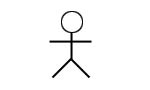
\includegraphics[width=0.7035in,height=0.698in]{chapter2-img1.jpg}  &
	\caption{FIGURECAPTION}
\end{figure}
Use case actor. Represents a user group\\\hline
\begin{figure}[h!]
	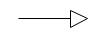
\includegraphics[width=0.4535in,height=0.9138in]{chapter2-img2.png}  &
	\caption{FIGURECAPTION}
\end{figure}
UML generalization arrow. Used to indicate inheritance. The
arrow's source, i.e.\ tail, represents the entity that
inherits from where the arrow points to.\\\hline
{\textless}{\textless}include{\textgreater}{\textgreater} &
UML stereotype to represent a mandatory extension to a
work{}-flow.\\\hline
{\textless}{\textless}extend{\textgreater}{\textgreater} &
UML stereotype to indicate that if certain conditions are met in a flow,
the entity to which this arrow points to can extend the
workflow.\\\hline
\end{supertabular}
\end{table}

The purpose of the use case diagrams is to give a clear overview of what
users shall be able to accomplish from our system. Furthermore, use
case diagrams are easier to communicate to external parties, such that
it is easier to agree on the system's properties. The
use case diagrams were used early in development to agree on the
requirements specification and to communicate to the supervisor what we
were trying to accomplish.

\begin{figure}[h!]
	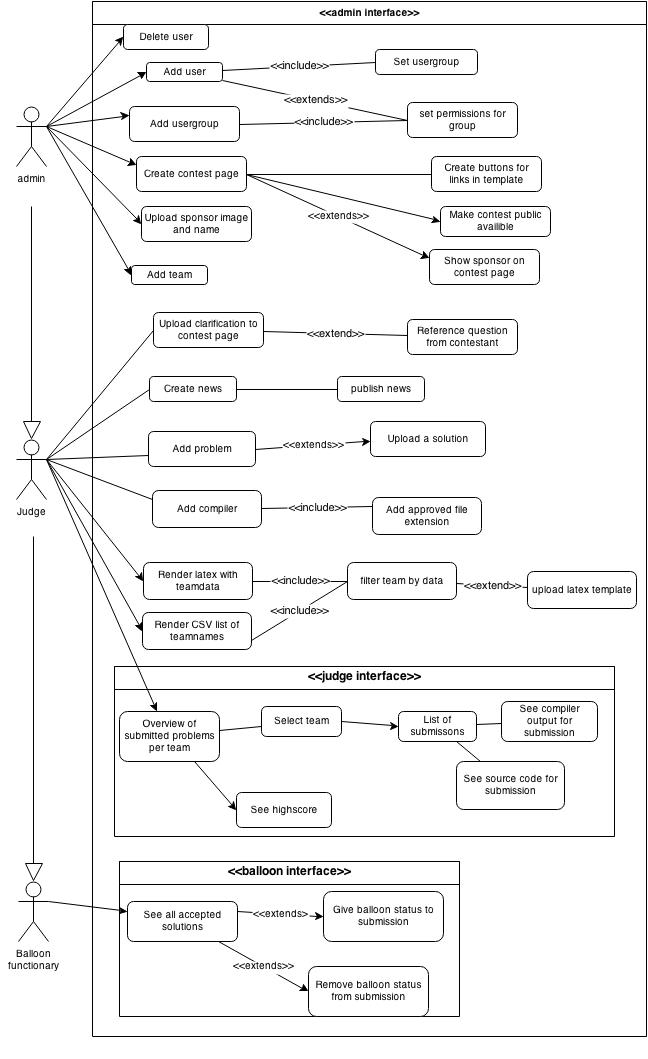
\includegraphics[width=5.8339in,height=9.5366in]{chapter2-img3.jpg} 
	\caption{FIGURECAPTION}
\end{figure}
As seen in figure X.X, admins has privileges to perform the actions of
any other group, in addition to their own set of actions. Thus,
membership in the admin group gives a user complete control in the
application domain. Furtherly, it can be noted that all usergroups have
the opportunity to act as a contestant to review the website.
Privileged users will are still restricted from appearing in the
official high score tables to prevent them from assuming a competing
role. This was to avoid the chance of any person with access to the
solutions to compete.







